\documentclass{standalone}
\usepackage{ tikz }
\usepackage{ xparse }
\usepackage{../../../macros}

\begin{document}
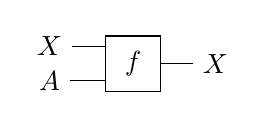
\begin{tikzpicture}[yscale=-1,x=1em,y=1.25em]

    \node (X1) at (0,0) {$X$};
    \node (A1) at (0,1) {$A$};
    \node (X2) at (6,0.5) {$X$};

    \node[draw, minimum height = 2em, minimum width = 2em, anchor = west, fill=white] at (2,0.5){$f$};

    \draw (X1) -- (2,0);
    \draw (A1) -- (2,1);

    \draw (4,0.5) -- (X2);


\end{tikzpicture}
\end{document}